\documentclass[tikz]{standalone}
\usepackage{tikz}
\usetikzlibrary{shapes, arrows, positioning}

\begin{document}
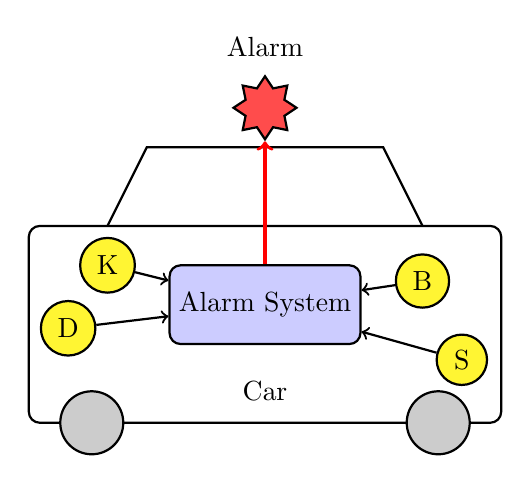
\begin{tikzpicture}[
    auto,
    node distance=1cm,
    thick
  ]

  % Styles
  \tikzstyle{sensor}=[draw, circle, minimum size=6mm, fill=yellow!80]
  \tikzstyle{system}=[draw, shape=rectangle, minimum width=2cm, minimum height=1cm, fill=blue!20, rounded corners]
  \tikzstyle{output}=[draw, shape=star, minimum size=8mm, fill=red!70, star points=8]

  % Car Body
  \draw[thick, rounded corners] (-3,-1) rectangle (3,1.5);
  \draw[thick] (-2,1.5) -- (-1.5,2.5) -- (1.5,2.5) -- (2,1.5);
  \draw[fill=black!20] (-2.2, -1) circle (0.4cm);
  \draw[fill=black!20] (2.2, -1) circle (0.4cm);
  \node at (0,-0.6) {Car};

  % Alarm System inside the car
  \node[system] (alarm) at (0, 0.5) {Alarm System};

  % Sensors positioned on the car
  \node[sensor] (K) at (-2, 1) {K}; % Key near steering wheel
  \node[sensor] (D) at (-2.5, 0.2) {D}; % Door
  \node[sensor] (S) at (2.5, -0.2) {S}; % Seat
  \node[sensor] (B) at (2, 0.8) {B}; % Battery in engine bay

  % Output (Alarm)
  \node[output] (A) at (0, 3) {};
  \node at (A.north) [above=1mm] {Alarm};


  % Arrows from sensors to alarm system
  \draw[->] (K) -- (alarm);
  \draw[->] (D) -- (alarm);
  \draw[->] (S) -- (alarm);
  \draw[->] (B) -- (alarm);

  % Arrow from alarm system to output
  \draw[->, very thick, red] (alarm) -- (A);

\end{tikzpicture}
\end{document}
